% biography section
% 
% If you have an EPS/PDF photo (graphicx package needed) extra braces are
% needed around the contents of the optional argument to biography to prevent
% the LaTeX parser from getting confused when it sees the complicated
% \includegraphics command within an optional argument. (You could create
% your own custom macro containing the \includegraphics command to make things
% simpler here.)
%\begin{IEEEbiography}[{\includegraphics[width=1in,height=1.25in,clip,keepaspectratio]{mshell}}]{Michael Shell}
% or if you just want to reserve a space for a photo:

\begin{IEEEbiography}[{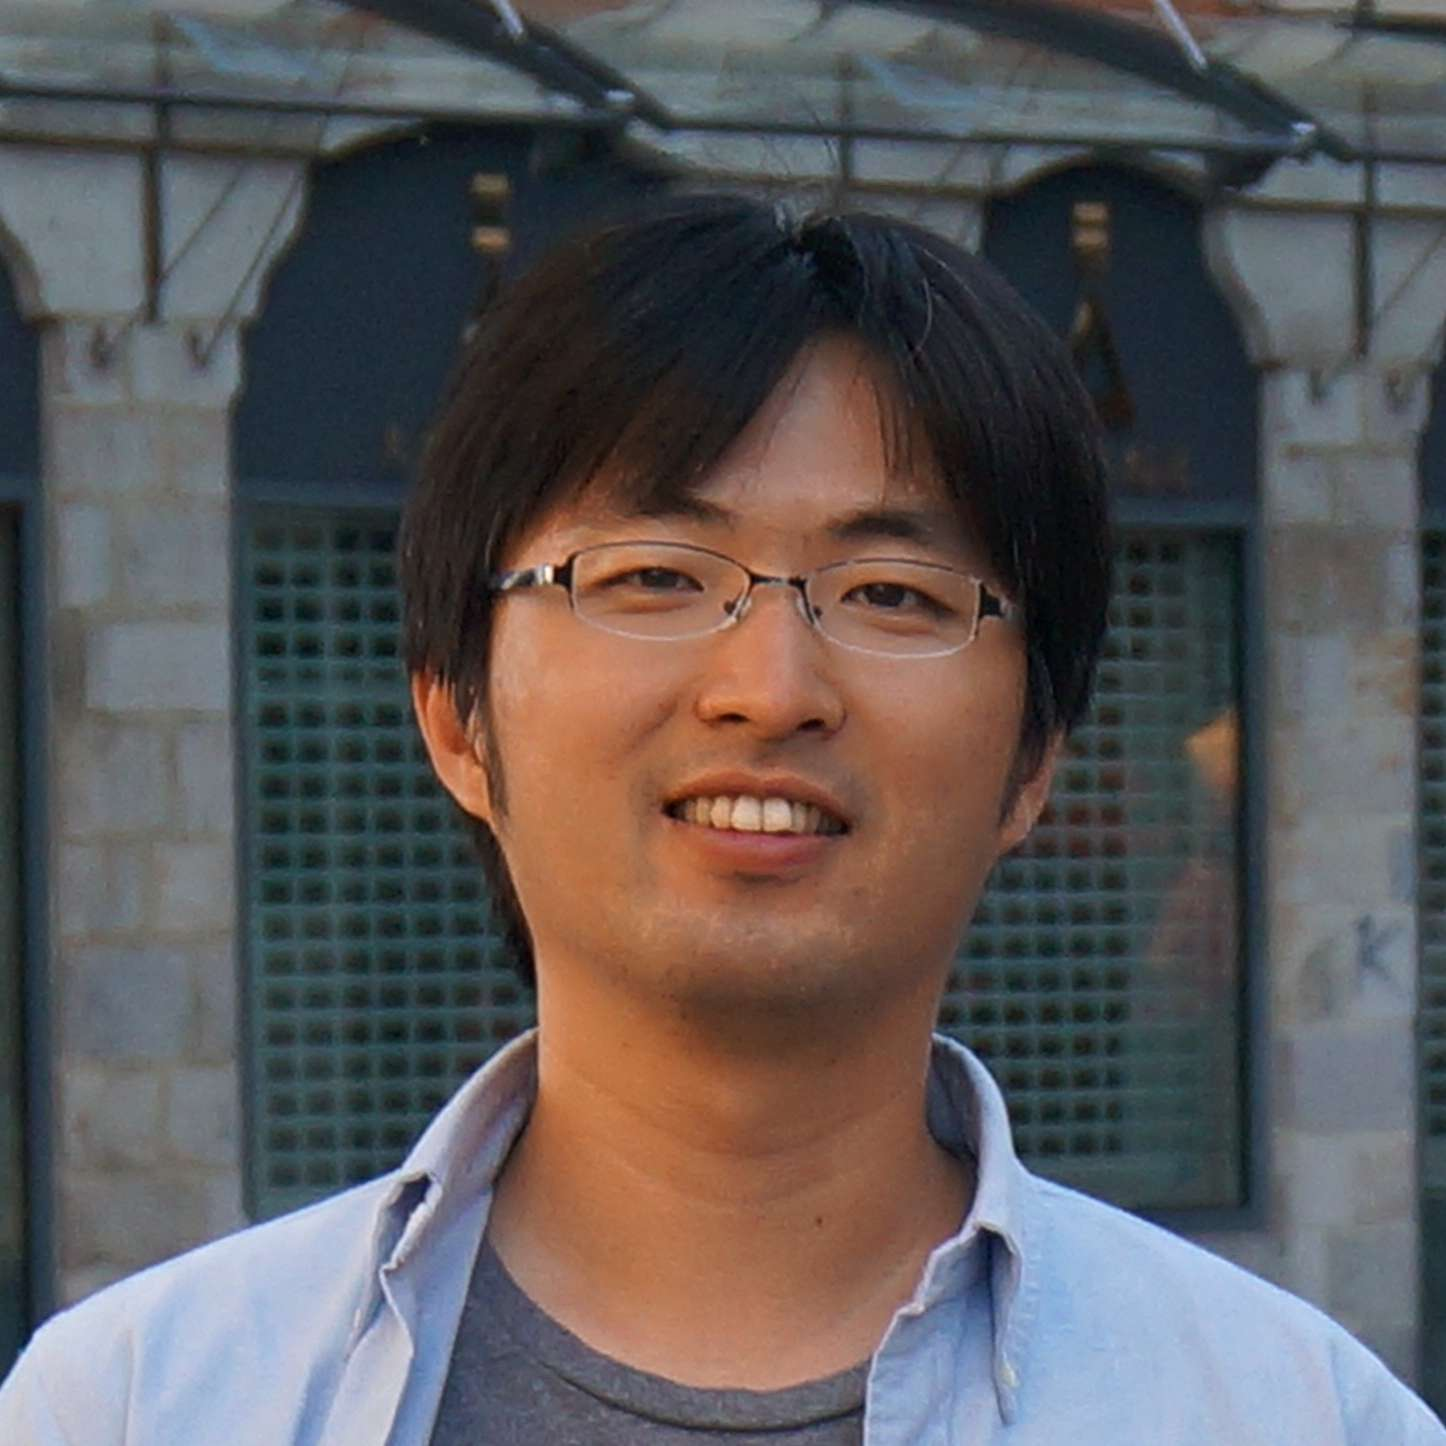
\includegraphics[width=1in,height=1.25in,keepaspectratio]{./fig/bio/jay.jpg}}]{Liang-Chieh Chen}
received his B.Sc. from National Chiao Tung University, Taiwan, his M.S. from the University of Michigan- Ann Arbor, and his
Ph.D. from the University of California- Los Angeles. He is currently working at Google. His research interests
include semantic image segmentation, probabilistic graphical models, and machine learning.
\end{IEEEbiography}

\begin{IEEEbiography}[{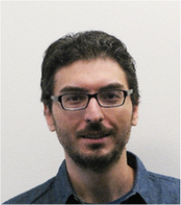
\includegraphics[width=1in,height=1.25in,keepaspectratio]{./fig/bio/gpapan.png}}]{George Papandreou}
(S'03--M'09--SM'14) holds a Diploma (2003) and a Ph.D. (2009) in Electrical
Engineering and Computer Science, both from the National Technical University
of Athens (NTUA), Greece. He is currently a Research Scientist at Google,
following appointments as Research Assistant Professor at the Toyota
Technological Institute at Chicago (2013-2014) and Postdoctoral Research Scholar
at the University of California, Los Angeles (2009-2013).

His research interests are in computer vision and machine learning, with a
current emphasis on deep learning. He regularly serves as a reviewer and
program committee member to the main journals and conferences in computer
vision, image processing, and machine learning. He has been a co-organizer of
the NIPS 2012, 2013, and 2014 Workshops on Perturbations, Optimization, and
Statistics and co-editor of a book on the same topic (MIT Press, 2016).
\end{IEEEbiography}

\begin{IEEEbiography}[{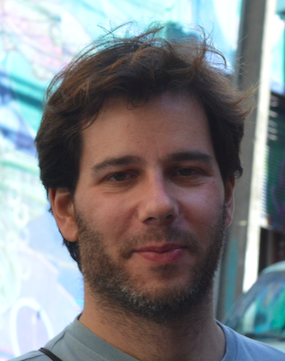
\includegraphics[width=1in,height=1.25in,keepaspectratio]{./fig/bio/iasonas.png}}]{Iasonas Kokkinos}
(S'02--M'06) obtained the Diploma of Engineering in 2001 and the Ph.D. Degree in 2006 from the School of Electrical and Computer Engineering of the National Technical University of Athens in Greece, and the Habilitation Degree in 2013 from Université Paris-Est. In 2006 he joined the University of California at Los Angeles as a postdoctoral scholar, and in 2008 joined as faculty the Department of Applied Mathematics of Ecole Centrale Paris (CentraleSupelec), working an associate professor in the Center for Visual Computing of CentraleSupelec and affiliate researcher at INRIA-Saclay. In 2016 he joined University College London and Facebook Artificial Intelligence Research. His currently research activity is on deep learning for computer vision, focusing in particular on structured prediction for deep learning, shape modeling, and multi-task learning architectures. He has been awarded a young researcher grant by the French National Research Agency, has served as associate editor for the Image and Vision Computing and Computer Vision and Image Understanding Journals, serves regularly as a reviewer and area chair for all major computer vision conferences and journals.
\end{IEEEbiography}

\begin{IEEEbiography}[{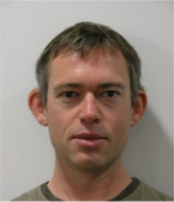
\includegraphics[width=1in,height=1.25in,keepaspectratio]{./fig/bio/kmurphy.png}}]{Kevin Murphy}
was born in Ireland, grew
up  in  England,  went  to  graduate  school  in  the
USA (MEng from U. Penn, PhD from UC Berkeley,
Postdoc at MIT), and then became a professor at
the Computer Science and Statistics Departments at
the University of British Columbia in
Vancouver, Canada in 2004. After getting tenure,
Kevin  went  to  Google  in  Mountain  View,  California
for his sabbatical. In 2011, he converted
to a full-time research scientist at Google. Kevin
has published over 50 papers in refereed conferences
and journals related to machine learning and graphical models.
He  has  recently  published  an  1100-page  textbook  called
``Machine Learning: a Probabilistic Perspective''
(MIT Press, 2012).
\end{IEEEbiography}

\begin{IEEEbiography}[{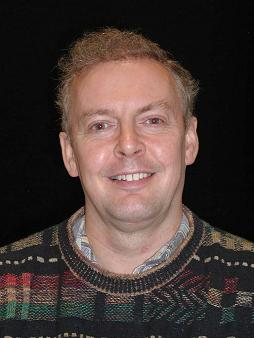
\includegraphics[width=1in,height=1.25in,keepaspectratio]{./fig/bio/alan.jpg}}]{Alan L. Yuille}
(F'09) received the BA degree in math-
ematics from the University of Cambridge in
1976. His PhD on theoretical physics, super-
vised by Prof. S.W. Hawking, was approved
in 1981. He was a research scientist in the
Artificial Intelligence Laboratory at MIT and
the Division of Applied Sciences at Harvard
University  from  1982  to  1988.  He  served
as  an  assistant  and  associate  professor  at
Harvard  until  1996.  He  was  a  senior  research scientist at the Smith-Kettlewell Eye
Research Institute from 1996 to 2002. He joined the University of
California, Los Angeles, as a full professor with a joint appointment
in  statistics  and  psychology  in  2002, and computer  science  in  2007. 
He was appointed a Bloomberg Distinguished Professor at Johns Hopkins University in January 2016.
He holds a joint appointment between the Departments of Cognitive science and Computer Science. 
His  research  interests  include
computational models of vision, mathematical models of cognition,
and artificial intelligence and neural network
\end{IEEEbiography}

%% \begin{IEEEbiography}{Michael Shell}
%% Biography text here.
%% \end{IEEEbiography}

%% % if you will not have a photo at all:
%% \begin{IEEEbiographynophoto}{John Doe}
%% Biography text here.
%% \end{IEEEbiographynophoto}

%% % insert where needed to balance the two columns on the last page with
%% % biographies
%% %\newpage

%% \begin{IEEEbiographynophoto}{Jane Doe}
%% Biography text here.
%% \end{IEEEbiographynophoto}

%% % You can push biographies down or up by placing
%% % a \vfill before or after them. The appropriate
%% % use of \vfill depends on what kind of text is
%% % on the last page and whether or not the columns
%% % are being equalized.

%% %\vfill

%% % Can be used to pull up biographies so that the bottom of the last one
%% % is flush with the other column.
%% %\enlargethispage{-5in}
